% sos2cayley astar_bomega.sos --rename a=a,!a=b
% Generated by sosl.sos.viz. Every visual choice is in the \tikzset below:
% edit a style to restyle, edit a coordinate to move a node.
\documentclass[tikz,border=4pt]{standalone}
\usepackage{amssymb}
\usetikzlibrary{arrows.meta,shapes.misc}
\begin{document}
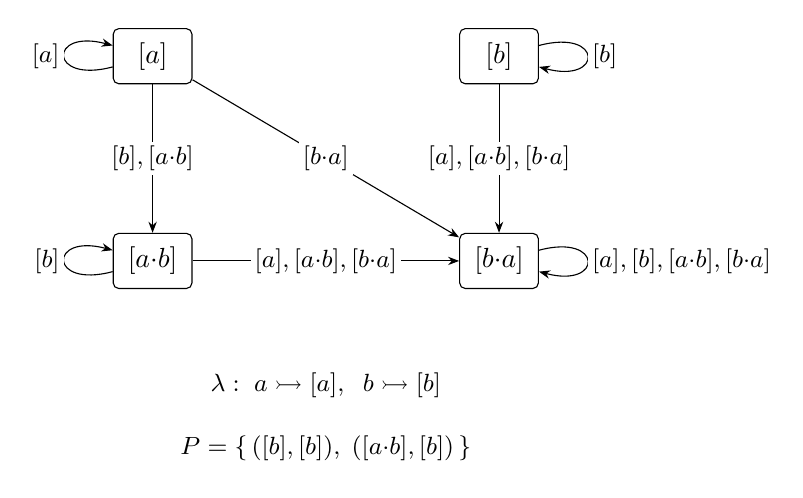
\begin{tikzpicture}[
  class/.style     = {draw, thin, rounded corners=2pt, inner sep=3pt,
                      minimum width=10mm, minimum height=7mm},
  root/.style      = {},          % the root needs no ink: the init stub says it
  init/.style      = {semithick, -{Stealth[length=4pt,width=3pt]}},
  arrow/.style     = {thin, -{Stealth[length=4pt,width=3pt]}},
  lbl/.style       = {font=\small, inner sep=1.5pt, fill=white},
  pairs/.style     = {anchor=north, font=\small},
]

  \node[class] (a) at (0.0,0.9) {$[a]$};
  \node[class] (b) at (4.4,0.9) {$[b]$};
  \node[class] (ab) at (0.0,-1.7) {$[a{\cdot}b]$};
  \node[class] (ba) at (4.4,-1.7) {$[b{\cdot}a]$};

  \draw[arrow] (a) to[loop left] node[lbl] {$[a]$} (a);
  \draw[arrow] (a) to node[lbl] {$[b],[a{\cdot}b]$} (ab);
  \draw[arrow] (a) to node[lbl] {$[b{\cdot}a]$} (ba);
  \draw[arrow] (b) to node[lbl] {$[a],[a{\cdot}b],[b{\cdot}a]$} (ba);
  \draw[arrow] (b) to[loop right] node[lbl] {$[b]$} (b);
  \draw[arrow] (ab) to node[lbl] {$[a],[a{\cdot}b],[b{\cdot}a]$} (ba);
  \draw[arrow] (ab) to[loop left] node[lbl] {$[b]$} (ab);
  \draw[arrow] (ba) to[loop right] node[lbl] {$[a],[b],[a{\cdot}b],[b{\cdot}a]$} (ba);

  \node[pairs] at (2.2,-3.0) {$\lambda:\; a \rightarrowtail [a],\;\; b \rightarrowtail [b]$};
  \node[pairs] at (2.2,-3.8) {$P = \{\, ([b],[b]),\; ([a{\cdot}b],[b]) \,\}$};
\end{tikzpicture}
\end{document}
